\documentclass[popl.tex]{subfiles}
\begin{document}

\section{Measuring the language intersection}\label{sec:measurement}

We will now attempt to put a probability distribution over the language intersection. We shall start with a few cursory but illustrative approaches, then proceed towards a more refined solution.

\subsection{Mode collapse}

Ordinarily, one might think to train a top-down PCFG sampler using a treebank of well-formed code snippets, however this method is highly degenerate in the finite case, exhibiting poor sample diversity. Consider an illustrative pathological case for top-down ancestral (TDA) sampling:
$$
G=\left\{ S \rightarrow A\:B \: \left(\frac{10^5 - 1}{10^5}\right), \hspace{2pt}
     S \rightarrow C\:C \: \left(\frac{1}{10^5}\right), \hspace{2pt}
     A \rightarrow a \: (1), \hspace{2pt}
     B  \rightarrow b \: (1), \hspace{2pt}
     C  \rightarrow a \: \left(\frac{1}{26}\right) \mid \ldots \mid z \: \left(\frac{1}{26}\right)\right\}
$$
Such a sampler will almost always yield $a b$, but most of $\mathcal{L}(G)$ is concealed in the hidden branch, $S \rightarrow C C$. Though a contrived example, it illustrates why TDA sampling is unviable: our sampler should match the true distribution over the finite CFL, not the PCFG's local approximation thereof.

\subsection{Exact enumeration}

To correct for mode collapse, a brute force solution would be to simply generate every tree. While the whole set can be materialized in some cases when the intersection language is small, this strategy is clearly suboptimal in the worst-case. Nevertheless, it is useful for checking completeness.

\begin{theorem}[Enumeration]\label{thm:enumeration}
  We will first denote the number of unique trees in a regex as $|e|$:
  \begin{equation}
    |e|: E \rightarrow \mathbb{N} = \begin{cases}
        1           & \text{if } e \in \Sigma \\
        x \times z  & \text{if } e = x \cdot z \\
        x + z       & \text{if } e = x \vee z
    \end{cases}
  \end{equation}
  To enumerate, we construct a bijection between trees and integers, then invoke $\bigcup_{i = 0}^{|R|}\big\{\texttt{enum}(R, i)\big\}$:
  \begin{equation}
    \texttt{enum}(e, n): E \times \mathbb{N} \rightarrow \Sigma^* = \begin{cases}
         e &\text{if } e \in \Sigma \\
         \texttt{enum}\big(x, \lfloor \frac{n}{|z|} \rfloor\big) \cdot \texttt{enum}\big(z,\, n \bmod |z|\big)  &\text{if } e = x \cdot z \\
         \texttt{enum}\big((x, z)_{\min(1, \lfloor\frac{n}{|x|}\rfloor)}, n-|x|\min(1, \lfloor\frac{n}{|x|}\rfloor)\big) &\text{if } e = x \vee z
    \end{cases}
  \end{equation}
\end{theorem}

This can be converted to a uniform sampler by drawing integers without replacement using a pseudorandom number generator, however, if $|e|$ is very large, \texttt{enum} can fail to capture modes.

\subsection{The problem with ambiguity}

The main problem with Thm.~\ref{thm:enumeration} is that it counts distinct trees, which overcounts the number of words, $|\mathcal{L}(G_\cap)|$. Since the Levenshtein automaton can be ambiguous, uniform tree sampling causes certain repairs to be overrepresented, resulting in a pernicious bias. Consider, for example,

\begin{lemma}\label{lemma:ambiguity}
If the FSA, $\alpha$, is ambiguous, then the intersection grammar, $G_\cap$, can be ambiguous.
\end{lemma}

\begin{proof}
Let $\ell$ be the language defined by $G=\{S\rightarrow LR, L \rightarrow\texttt{(}, R \rightarrow\texttt{)}\}$, where $\alpha=L(\err\sigma, 2)$, the broken string $\err\sigma$ is $\texttt{)(}$, and $\mathcal{L}(G_\cap) = \ell \cap \mathcal{L}(\alpha)$. Then, $\mathcal{L}(G_\cap)$ contains the following two identical repairs: \texttt{\hlred{)}(\hlgreen{)}} with the parse $S \rightarrow q_{00}Lq_{21}\phantom{.}q_{21}Rq_{22}$, and \texttt{\hlorange{(}\hlorange{)}} with the parse $S \rightarrow q_{00}Lq_{11}\phantom{.}q_{11}Rq_{22}$.
\end{proof}

\noindent We would expect the underlying sample space to be a proper set, \textit{not} a multiset. If we are to sample repairs uniformly at random, ambiguity cannot be permitted. To obtain the exact normalizing constant and disambiguate $\ell_\cap$, we require a different representation which will now be described.

\subsection{Disambiguation}\label{sec:transfer_method}

To count the number of distinct repairs, we will need to convert $G_\cap$ to an automaton. Since $\mathcal{L}(G_\cap)$ is finite, it must be regular a fortiori. Recalling the definition for an NFA, $\langle Q, \Sigma, \delta, q_\alpha: Q, F \subseteq Q \rangle$, and star-free regex, $e \rightarrow \Sigma \mid e \cdot e \mid e \lor e$, we will proceed by structural induction on the regex:
\begin{equation*}
N(e) =
\begin{cases}
  \begin{alignedat}{8}
    &\big\langle \{q_\alpha, q_\omega\}
    &&\,,\, \{ q_\alpha \overset{e}{\rightarrow} q_\omega \}
    &&\,,\, q_\alpha\,\,, \{q_{\omega}\}
    &&\big\rangle
    &&\:\: \text{if } e \in \Sigma \\[0.5em]

    &\big\langle Q_{x} \cup Q_{z}
    &&\,,\, \{ q \overset{s}{\rightarrow} q_{\alpha z} \mid (q \overset{s}{\rightarrow} q_{\omega}^{\in F_x}) \in \delta_x \} \cup \delta_{x} \cup \delta_{z}
    &&\,,\, q_{\alpha x}\,, F_{z}
    &&\big\rangle
    &&\:\: \text{if } e = x \cdot z \\[0.5em]

    &\Bigg\langle   \begin{matrix} Q_{x}\cup \{q_{\alpha e}\}\:\cup\\ Q_{z} \cup \{q_{\omega e}\}\phantom{\:\cup} \end{matrix}
    &&\,,\, \begin{matrix}\{ q_{\alpha e} \overset{s}{\rightarrow} q \mid (q_{\alpha x, \alpha z} \overset{s}{\rightarrow} q)\in \delta_{x, z} \} \cup \delta_{x}\:\cup\\
    \{ q \overset{s}{\rightarrow} q_{\omega e} \mid (q \overset{s}{\rightarrow} q_{\omega}^{\in F_{x,z}})\in \delta_{x, z} \}\cup \delta_{z}\phantom{\,\:\cup}\end{matrix}
    &&\,,\, q_{\alpha e}\,, \{q_{\omega e}\}
    &&\Bigg\rangle
    &&\:\:\text{if } e = x \lor z\hspace{-0.5cm}\\[-0.5em]
    \multicolumn{9}{c}{\tiny{\text{- - - - - - - - - - - - or - - - - - - - - - - - -}}} \\[-0.5em]
    &\big\langle Q_{x} \cup Q_{z} \cup \{q_{\alpha e}\}
    &&\,,\, \{ q_{\alpha e} \overset{s}{\rightarrow} q \mid (q_{\alpha x, \alpha z} \overset{s}{\rightarrow} q) \in \delta_{x, z} \}  \cup \delta_{x} \cup \delta_{z}
    &&\,,\, q_{\alpha e}\,, F_{x} \cup F_{z}
    &&\big\rangle
    &&\:\: \text{if } e = x \lor z
  \end{alignedat}
\end{cases}\vspace{0.2cm}
\end{equation*}
Though less conventional than Thompson's construction, $N(e)$ avoids the creation of unnecessary $\varepsilon$ arcs. And while slightly more verbose, we find the topology induced by the first version of the $\lor$ case to be more favorable for minimization. Continuing with our running example from \S~\ref{sec:repair_ex}, we will use Brzozowski's algorithm~\cite{brzozowski1962canonical} to construct the unique minimal DFA, $D^*_\cap \equiv_\mathcal{L} G_\cap$: \vspace{-0.4cm}

\begin{figure}[H]
  \centering
  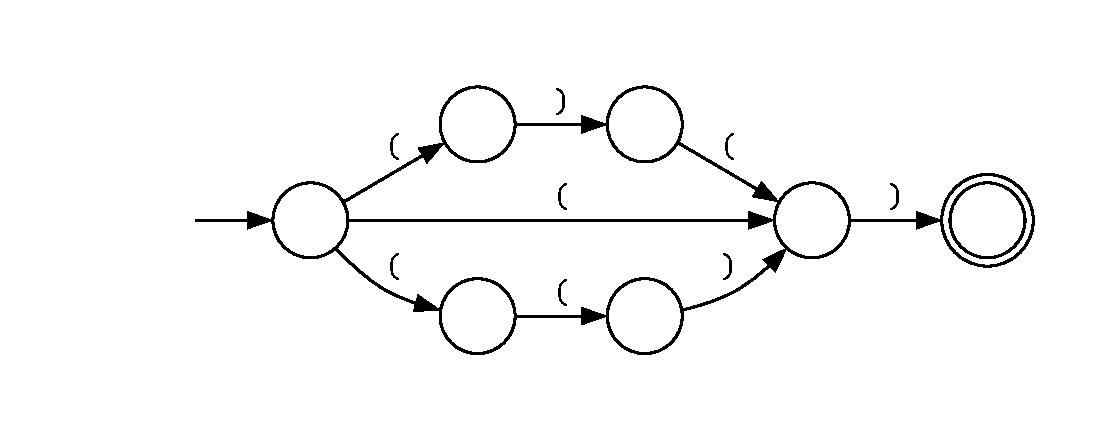
\includegraphics[width=0.27\textwidth]{figures/dyck_nfa}
  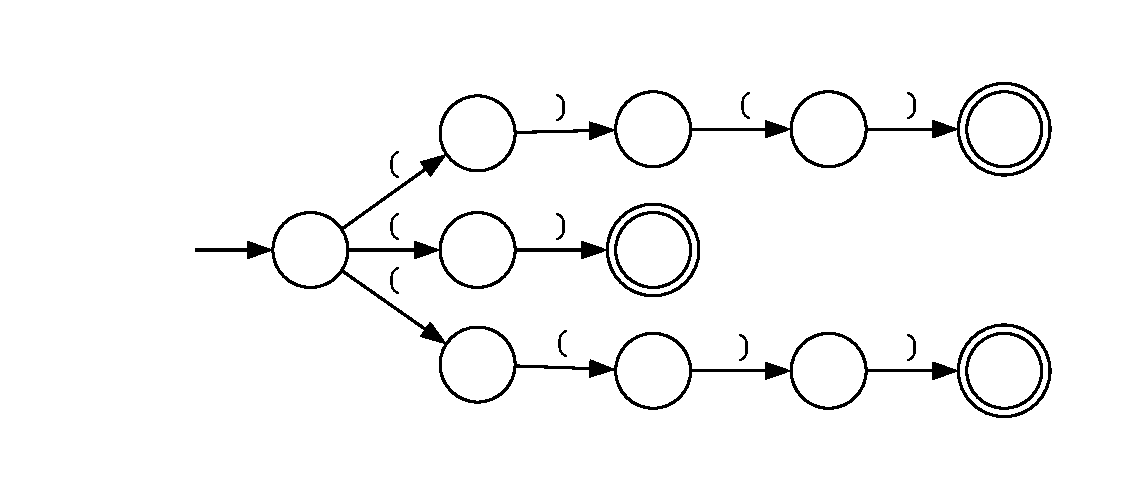
\includegraphics[width=0.27\textwidth]{figures/dyck_nfa_orig}
  
\includegraphics[width=0.30\textwidth]{figures/dyck_dfa}
  \vspace{-0.2cm}
  \caption{FSA for $\mathcal{L}\big(L(\texttt{())}, 1)\big)\cap\mathcal{L}(G')$ (a) with or (b) without $\lor$-merging, and then (c) post-minimization.}\label{fig:fsas_for_re}
  \vspace{-0.2cm}
\end{figure}
Since $\mathcal{L}(G_\cap)$ is necessarily finite, we can infer that the corresponding DFA is acyclic and thus representable as an upper triangular adjacency matrix under a topological ordering of $\delta$. For any such DFA, we can ascertain the size of its language by counting walks from $q_\alpha$ to $q_\omega \in F$. Letting $A$ be the adjacency matrix for $D_\cap^*$, i.e., $A[q, q'] = \big[1 \text{ if } \exists s: \Sigma \text{ s.t. } (q \overset{s}{\rightarrow} q') \in \delta \text{ else } 0\big]$, the number of words it recognizes is given via the transfer matrix method~\cite{flajolet2009analytic}, that is,
\begin{align}
  C(A, q_\alpha, F): \mathbb{N}^{|Q|\times|Q|} \times Q \times 2^Q \rightarrow \mathbb{N} = \sum_{\mathclap{q_\omega \in F}}(I-A)^{-1}[q_\alpha, q_\omega] &= \sum_{\mathclap{q_\omega \in F}}\sum_{i = 0}^{\mathclap{|Q|-1}}A^i[q_\alpha, q_\omega]
\end{align}
\noindent Plugging in powers of the adjacency matrix for the DFA shown in Fig.~\ref{fig:fsas_for_re}.(c), we arrive at the total:
\begin{align}
(I-A)^{-1} &= \hspace{1cm}I + A \hspace{1cm}+\hspace{1.05cm} A^2 \hspace{1.07cm}+\hspace{1cm} A^3 \hspace{0.9cm}+\hspace{0.9cm} A^4\\
  &=\begin{tiny}\begin{pmatrix}
      1 & 1 &   &   &   &   \\
        & 1 & 1 & 1 &   &   \\
        &   & 1 &   & 1 &   \\
        &   &   & 1 & 1 &   \\
        &   &   &   & 1 & 1 \\
        &   &   &   &   & 1  \\
  \end{pmatrix} + \begin{pmatrix}
        &   & 1 & 1 &   &   \\
        &   &   &   & 2 &   \\
        &   &   &   &   & 1 \\
        &   &   &   &   & 1 \\
        &   &   &   &   &   \\
        &   &   &   &   &   \\
  \end{pmatrix} + \begin{pmatrix}
        &   &   &   & 2 &   \\
        &   &   &   &   & 2 \\
        &   &   &   &   &   \\
        &   &   &   &   &   \\
        &   &   &   &   &   \\
        &   &   &   &   &   \\
  \end{pmatrix} + \begin{pmatrix}
        &   &   &   &   & 2 \\
        &   &   &   &   &   \\
        &   &   &   &   &   \\
        &   &   &   &   &   \\
        &   &   &   &   &   \\
        &   &   &   &   &   \\
  \end{pmatrix}\end{tiny}\\
  &= \begin{tiny}\begin{pmatrix}
    1   & 1  & 1  & \underline{1} & 2 & \underline{2} \\
        & 1  & 1  & 1 & 2 & 2 \\
        &    & 1  &   & 1 & 1 \\
        &    &    & 1 & 1 & 1 \\
        &    &    &   & 1 & 1 \\
        &    &    &   &   & 1 \\
\end{pmatrix}\end{tiny} \text{ therefore, } \big|\mathcal{L}(D_\cap^*)\big| = C\big(A, q_0, \{q_3, q_5\}\big) = \underline{1} + \underline{2} = 3.
\end{align}
Note the model counting problem for arbitrary REs is strictly harder than deciding intersection nonemptiness as it requires determinization, however, weak bounds may be obtained by applying $C$ to the FSA generated by $N(e)$ or by direct analysis of $e$. While the inequality $C_{D_\cap^*} \leq C_{N(e)} \leq |e|$ will hold, the bounds provided by the latter approximations may be vacuous, whereas $C_{D_\cap^*}$ is exact. $D_\cap^*$ may be enumerated by standard methods~\cite{flajolet2009analytic} and sampled uniformly with a suitable PRNG.
\ifSubfilesClassLoaded{\par\clearpage\bibliography{../bib/acmart}}{}
\end{document}
